\documentclass[10pt]{beamer}

\mode<presentation>
{
  \usetheme[height=1.25cm]{Madrid}
  \setbeamertemplate{navigation symbols}{}
  \setbeamercolor{alerted text}{fg=illini}
}
\usebackgroundtemplate{
\includegraphics[width=\paperwidth,height=\paperheight]{uc-background}}

\usepackage[english]{babel}
\usepackage{epsfig,subfigure,bm}
\usepackage{multimedia}
\usepackage{psfrag}
\usepackage{animate}

%%%%%% Begin of my macros and options

\setbeamertemplate{section in toc shaded}[default][55]
\setbeamertemplate{subsection in toc shaded}[default][55]
\setbeamercolor{block title}{fg=white,bg=illini}
\setbeamercolor{block body}{fg=black,bg=mygrey}

\setbeamercolor{emphprimary}{fg=CBlue}
\setbeamercolor{emphsecondary}{fg=illini}
\setbeamercolor{emphtertiary}{fg=mygreen}
\definecolor{darkForestGreen}{rgb}{.1,1,.1}
\definecolor{veryLightGray}{rgb}{.9,.9,.9}
\definecolor{greenApple}{rgb}{.3,.9,.3}

\setbeamercolor{frametitle}{bg=CBlue}   
\setbeamercolor{title}{bg=CBlue}

\usepackage{amsmath,amssymb,amsxtra,amsthm}
\usepackage{algorithm,algorithmic}
\usepackage{natbib}
\usepackage{bibentry}
\usepackage{xspace}
\usepackage{changepage}

\pdfmapfile{+sansmathaccent.map}

\definecolor{myblue}{rgb}{.2,.2,.7}
\definecolor{myred}{rgb}{.7,.2,.2}
\definecolor{mygreen}{rgb}{.2,.7,.2}
\definecolor{mygrey}{rgb}{0.9,0.9,0.9}
\definecolor{CBlue}{cmyk}{1,0.25,0,0}
\definecolor{illini}{rgb}{0.98,0.4,0.05}
\definecolor{black}{cmyk}{0,0,0,1}

\newcommand{\myemph}[1]{{\usebeamercolor[fg]{emphprimary}
    \textbf{#1}}}
\newcommand{\myemphalt}[1]{{\usebeamercolor[fg]{emphsecondary}
    \textbf{#1}}}

\graphicspath{{figs/}}

\title[Math for Robotics] % (optional, use only with long paper titles)
{CSE276C - Root Finding}

\author[H.~I. Christensen] % (optional, use only with lots of authors)
{Henrik I.~Christensen}
% - Give the names in the same order as the appear in the paper.  -
% Use the \inst{?} command only if the authors have different
% affiliation.

\AtBeginSection[]
{
   \begin{frame}
       \frametitle{Outline}
       \tableofcontents[currentsection]
   \end{frame}
}

\institute[UCSD] % (optional, but mostly needed)
{
  \begin{minipage}[c]{.2\textwidth}
    
\includegraphics[width=.65\linewidth]{ucsealnew}%
  \end{minipage}%
  \begin{minipage}[c]{.6\textwidth}
    \small
%%    \begin{center}
      Computer Science and Engineering\\
      University of California, San Diego\\
      \myemph{\url{http://cri.ucsd.edu}}\\          
%%    \end{center}

  \end{minipage}
%%  \vspace*{1ex}
}
%% - Use the \inst command only if there are several affiliations.
%% - Keep it simple, no one is interested in your street address.

\bigskip

\date[Oct 2024]% (optional, should be abbreviation of conference name)
{\small%
  October 2024}

\begin{document}
  
\nobibliography{/Users/hic/Dropbox/bibliography/bib-file}
\bibliographystyle{plain}

\begin{frame}[plain]
  \titlepage
\end{frame}

\section{Introduction}

\begin{frame}
  \frametitle{Introduction}
  \begin{itemize}
  \item Root finding or detection of zero-crossings, i.e., f(x) = 0
  \item Numerous applications in robotics
    \begin{enumerate}
    \item Numerical solution to inverse kinematics
    \item Collision detection in planning and navigation
    \item Detection of optimal control strategies
    \end{enumerate}
  \item Two main cases:
    \begin{enumerate}
    \item Non-linear systems
    \item Polynomial systems - factorization
    \end{enumerate}
  \end{itemize}
\end{frame}

\section{Bracketing}

\begin{frame}
  \frametitle{Braketing}
  \begin{itemize}
  \item First problem is to know where to look for roots. 
  \item What would be your strategy? \pause
  \item Can we identify an interval $[a,b]$ where f(x) changes sign, i.e:
    \[
      f(a) f(b) < 0
    \]
  \item Once we have an interval/bracket we can refine the strategy
  \item Good strategies?
    \begin{itemize}
    \item Hill climbing/decent
    \item Sampling
    \item Model information
    \end{itemize}
  \end{itemize}
\end{frame}

\begin{frame}
  \frametitle{Bracketing}
  \begin{columns}
    \begin{column}{4.8cm}
      \begin{itemize}
      \item Consider this function, what would be your strategy? 
      \end{itemize}
    \end{column}
    \begin{column}{4.5cm}
      \centerline{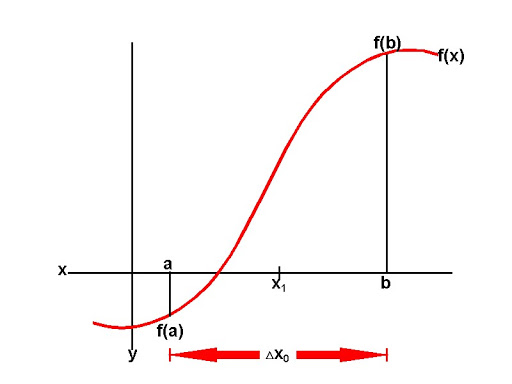
\includegraphics[width=4cm]{example-function}}
    \end{column}
  \end{columns}
\end{frame}

\subsection{Bi-section}

\begin{frame}
  \frametitle{Bisection}
  \begin{itemize}
  \item Given a, b, f(a), f(b) evaluate f at
    \[
      c = \frac{a+b}{2}
    \]
    decision
    \[
      \begin{array}{ccc}
        f(a) f(c) < 0 &?& \left\{
                          \begin{array}{cc}
                            Yes & I_{new} = [a,c]\\
                            No & I_{new} = [c,b]\\
                          \end{array}\right. \\

      \end{array}
    \]
  \end{itemize}
\end{frame}

\begin{frame}
  \frametitle{Bisection convergence}
  \begin{itemize}
  \item The interval size is changing
    \[
      s_{n+1} = \frac{s_n}{2}
    \]
  \item number of evaluations is
    \[
      n = \log_2 \frac{s_0}{s}
    \]
  \item Convergence is considered {\bf linear} as
    \[
      s_{n+1} = \mbox{ const } s_n^m
    \] with m = 1. 
  \item When $m>1$ convergence is termed super linear
  \end{itemize}
\end{frame}


\subsection{Secant}

\begin{frame}
  \frametitle{Secant Method}
  \begin{itemize}
  \item If you have a smooth function. Take a, b, f(a), f(b)
  \item Computer intersection point
  \end{itemize}
  \begin{columns}
    \begin{column}{7cm}
      \[
        \Delta = \frac{f(a) - f(b)}{a - b}
      \]
      \[
        c \Delta + f(a) = 0 \Leftrightarrow c = \frac{-f(a)}{\Delta}
      \] so d = a+c \\
    repeat for convergence
    \end{column}
    \begin{column}{4cm}
      \centerline{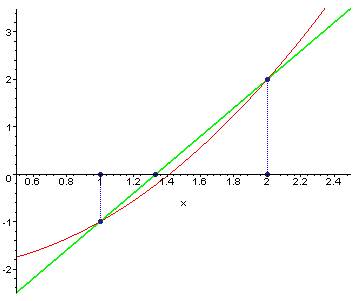
\includegraphics[width=3.9cm]{Secant_method}}
    \end{column}
  \end{columns}
\end{frame}

\begin{frame}
  \frametitle{Secant Method}
  \begin{itemize}
  \item The Secant Method is not gauranteed to pick the two points with opposite sign
  \item Secant is super-linear with a convergence rate of
    \[
      \lim_{k \rightarrow \infty} |s_{k+1}| = const |s_k|^{1.618}
    \]
  \item When could we be in trouble? \pause
  \item When you have major changes in the 2nd derivative close to root
  \end{itemize}
\end{frame}

\subsection{Regula Falsi / False Position}

\begin{frame}
  \frametitle{Regula Falsi / false position}
  \begin{itemize}
  \item Principle similar to Secant
  \item Always choose the interval with end-point of opposite sign
  \item Regula-falsi also has super-linear convergence, but harder to show
  \end{itemize}
\end{frame}

\section{Root Finding}

\subsection{Brent's Method}

\begin{frame}
  \frametitle{Brent's Method}
  \begin{itemize}
  \item We can leverage methods from interpolation theory
  \item Assume we have three points  (a, f(a)), (b, f(b)), (c, f(c))
  \item We can leverage Lagrange's method
    \[
      \begin{array}{cc}
      x = &  \frac{(y-f(a))(y-f(b)) c}{(f(c)-f(a))(f(c)-f(b))} +\\
          &  \frac{(y-f(b))(y-f(c)) a}{(f(a)-f(b))(f(a)-f(c))} +\\
          &  \frac{(y-f(c))(y-f(a)) b}{(f(b)-f(c))(f(b)-f(A))}\\
      \end{array}
    \]
  \item if we set y = 0 and solve for x we get
    \[
      x = b + \frac{P}{Q}
    \]
  \end{itemize}
\end{frame}

\begin{frame}
  \frametitle{Brent's Method (cont)}
  \begin{itemize}
  \item such that
    \[
      \begin{array}{cc}
        P = &  S(T(R-T)(c-b) - (1-R)(b-a))\\
        Q = & (T-1)(R-1)(S-1)\\
      \end{array}
    \]
  \item where R = f(b)/f(c), S = f(b)/f(a), T = f(a)/f(c)
  \item So b is expected to be ``the estimate'' and $\frac{P}{Q}$ is a correction term.
  \item When $\frac{P}{Q}$ is too small it is replaced by a bi-section step
  \item Brent is generally considered the recommended method. 
  \end{itemize}
\end{frame}

\subsection{Newton-Raphson's Method}

\begin{frame}
  \frametitle{Newton Rapson's Method }
  \begin{itemize}
  \item How can we use access to 1st order gradient information?
  \item For well behaved functions we can use a Taylor approximation
    \[
      f(x + \delta) \approx f(x) + f'(x) \delta + \frac{f''(x)}{2} \delta^2 + \ldots
    \]
  \item for a small $\delta$ and well behaved functions higher order terms are small
  \item if $f(x + \delta)$ = 0 we have
    \[
      \begin{array}{rl}
        f(x) + f'(x) \delta & = 0 ~~~ \Leftrightarrow \\ 
                     \delta & = -\frac{f(x)}{f'(x)}\\
      \end{array}
    \] 
  \item A search strategy is then
    \[
      x_{n+1} = x_n - \frac{f(x_n)}{f'(x_n)}
    \]
  \end{itemize}
\end{frame}

\begin{frame}
  \frametitle{Newton-Raphson - Notes}
  \begin{itemize}
  \item In theory one can approximate the gradient
    \[
      f'(x) = \frac{f(x+dx) - f(x)}{dx}
    \]
  \item For many cases this may not be a good approach
    \begin{enumerate}
    \item for $\delta >> 0$ the linearity assumption is weak
    \item For $\delta \approx 0$ the numerical accuracy can be challenging
    \end{enumerate}
  \end{itemize}
\end{frame}

\begin{frame}
  \frametitle{Multi-variate Newton Raphson}
  \begin{itemize}
  \item What is we have to solve
    \[
      \begin{array}{rcl}
        f(x,y) & = & 0 \\
        g(x,y) & = & 0 \\
      \end{array}
    \]
  \item A simple example
    \[
      f_i (x_0, x_1, \ldots, x_{n-1}) \mbox { ~~~~ } i = 0, ..., n-1
    \]
    we get
    \[
      f_i(\vec{x} + \delta \vec{x}) = f_i(\vec{x}) + \sum_{j=0}^{n-1} \frac{\partial f_i}{\partial x_j}\delta \vec{x} + O(\delta \vec{x}^2)
    \]
  \end{itemize}
\end{frame}

\begin{frame}
  \frametitle{Multi-variate case}
  \begin{itemize}
  \item The matrix of partial derivatives
    \[
      J_{ij} = \frac{\partial f_i}{\partial x_j}
    \]
  \item is termed the Jacobian. 
  \item We can now formulate
    \[
      f_i (\vec{x} + \delta\vec{x}) = f_j(\vec{x}) + J \delta \vec{x} + O(\delta\vec{x}^2)
    \]
  \item we can then as before rewrite
    \[
      J \delta \vec{x} = -f \mbox{ ~~ solve w. LU}
    \]
    or
    \[
      \vec{x}_{new} = \vec{x_{old}} + \delta \vec{x}
    \]
    for some cases an improved strategy is 
    \[
      \vec{x}_{new} = \vec{x_{old}} + \lambda \delta \vec{x}
    \] where $\lambda \in [0,1]$ to control convergence
  \end{itemize}
\end{frame}

\section{Search Summary}

\begin{frame}
  \frametitle{Search Summary}
  \begin{itemize}
  \item Simple search strategies for detect zeros / roots
  \item Bracketing is essential to determine the locations to search
  \item Brent's method in general robust strategy for root finding
  \item Newton-Raphson effective (for small $\delta$) and when gradient info is available
  \item Generalization in most cases is relative straight forward
  \end{itemize}
\end{frame}

\begin{frame}
  \frametitle{Questions}
  \centerline{\Huge Questions}
\end{frame}

\begin{frame}[plain]
  \frametitle{Roots of polynomials}
  \centerline{\Huge Roots of Polynomials}
\end{frame}

\section{Polynomial Roots - Introduction}

\begin{frame}
  \frametitle{Introduction}
  \begin{itemize}
  \item Earlier we looked at direct search for roots
  \item Bracketing was the way to limit the search domain
  \item Brent's method was a simple strategy to do search
  \item What if we have a polynomial?
    \begin{enumerate}
    \item Can we find the roots?
    \item Can we simplify the polynomial?
    \end{enumerate}
  \item Lets explore this
  \end{itemize}
\end{frame}

\section{Roots of Low Order Polynomials}

\begin{frame}
  \frametitle{Low order polynomials}
  \begin{itemize}
  \item We have closed form solutions to roots of polynomials up to degree 4
  \item Quadratics
    \[
      ax^2 + bx +c = 0, \mbox{~~~~} a\neq0
    \]
    has two roots
    \[
      x = \frac{-b \pm \sqrt{b^2 - 4ac}}{2a}
    \]
    we have real unique, dual or imaginary solutions
  \end{itemize}
\end{frame}

\begin{frame}
  \frametitle{Cubics}
  \begin{itemize}
  \item The cubic equation
    \[
      x^3 + px^2 + qx +r =0
    \] can be reduced using substitution
    \[
      x = y - \frac{p}{3}
    \] to the form
    \[
      y^3 +  a y + b = 0
    \] where
    \[
      \begin{array}{rcl}
        a &= & \frac{1}{3} (3q - p^2)\\
        b &= & \frac{1}{27} (2p^3 - 9 pq + 27r)\\
      \end{array}
    \] the condensed form has 3 roots
    \[
      \begin{array}{rcl}
        y_1& = & A+B\\
        y_2& = & -\frac{1}{2}(A+B) + \frac{i \sqrt{3}}{2} (A-B)\\
        y_3& = & -\frac{1}{2}(A+B) - \frac{i \sqrt{3}}{2} (A-B)\\
      \end{array}
    \] where
    \[
      \begin{array}{rclcrcl}
        A & = & \sqrt[3]{- \frac{b}{2} + \sqrt{\frac{b^2}{4} + \frac{a^3}{27}}} & \mbox {~~~} &
        B & = & \sqrt[3]{- \frac{b}{2} - \sqrt{\frac{b^2}{4} + \frac{a^3}{27}}}\\                                                                                                        
      \end{array}
    \]
  \end{itemize}
\end{frame}

\begin{frame}
  \frametitle{Cubic (cont)}
  \begin{itemize}
  \item We have three cases:
    \begin{enumerate}
    \item $\frac{b^2}{4} + \frac{a^3}{27} > 0$: one real root and two conjugate roots
    \item $\frac{b^2}{4} + \frac{a^3}{27} = 0$: three real roots of which at least two are equal
    \item $\frac{b^2}{4} + \frac{a^3}{27} < 0$: three real roots and unequal roots
    \end{enumerate}
  \end{itemize}
\end{frame}

\begin{frame}
  \frametitle{Quartics}
  \begin{itemize}
  \item For the equation
    \[
      x^4 + p x^3 + q x^2 + r x + s =0
    \] we can apply a similar trick
    \[
      x = y - \frac{p}{4}
    \]
    to get
    \[
      y^4 + a y^2 + b y + c = 0
    \]
    where
    \[
      \begin{array}{rcl}
        a& = & q - \frac{3p^2}{8}\\
        b& = & r + \frac{p^3}{8} - \frac{pq}{2}\\
        c& = & s - \frac{4p^4}{256} + \frac{p^2 q}{16} - \frac{pr}{4}\\
      \end{array}
    \]
  \end{itemize}
\end{frame}
\begin{frame}
  \frametitle{Quartics (cont.)}
  \begin{itemize}
  \item The reduced equation can be factorized into
    \[
      z^3 - q z^2 + (pr-4s) z + (4sq - r^2 - p^2s) = 0
    \]
    if we can estimate $z_1$ of the above cubic then
    \[
      \begin{array}{rcl}
        x_1 &= & -\frac{p}{4} + \frac{1}{2} (R+D) \\
        x_2 &= & -\frac{p}{4} + \frac{1}{2} (R-D) \\
        x_3 &= & -\frac{p}{4} - \frac{1}{2} (R+E) \\
        x_4 &= & -\frac{p}{4} - \frac{1}{2} (R-D) \\
      \end{array}
    \] where
    \[
      \begin{array}{rcl}  
        R &=& \sqrt{\frac{1}{4} p^2 - q + z_1} \\
        D &=& \sqrt{\frac{3}{4} p^2 - R^2 - 2Q + \frac{1}{4}(4pq - 8r - p^3) R^{-1}}\\
        E &=& \sqrt{\frac{3}{4} p^2 - R^2 - 2Q - \frac{1}{4}(4pq - 8r - p^3) R^{-1}}\\
      \end{array}
    \]
  \end{itemize}
\end{frame}


\section{Root Counting}

\begin{frame}
  \frametitle{Root Counting}
  \begin{itemize}
  \item Consider a polynomial of degree n:
    \[
      p(x) = a_n x^n + a_{n-1} x^{n-1} + \ldots + a_1 x + a_0
    \]
  \item if $a_i$ are real the roots are real or complex conjugate pairs. 
  \item p(x) has n roots
  \item Descartes rules of sign:
    \begin{itemize}
    \item ``The number of positive real zeroes in a polynomial
      function p(x) is the same or less than by an even numbers as the
      number of changes in the sign of the coefficients. The number of
      negative real zeroes of the p(x) is the same as the number of
      changes in sign of the coefficients of the terms of p(-x) or
      less than this by an even number''
    \end{itemize}
  \item Consider
    \[
      p(x) = x^5 + 4 x^4 - 3 x^2 + x -6
    \]
  \item So it must have 3 or 1 postive root and
  \item and it must have 2 or 0 negative roots
  \end{itemize}
\end{frame}

\begin{frame}
  \frametitle{Sturms theorem}
  \begin{itemize}
  \item We can derive a sequence of polynomials
  \item Let f(x) be a polynomial. Denote the original $f_0(x)$ and the
    derivative $f'(x) = f_1(x)$. Consider
    \[
      \begin{array}{rcl}
        f_0(x)      &=& q_1(x) f_1(x) - f_2(x) \\
        f_1(x)      &=& q_2(x) f_2(x) - f_3(x) \\
                 &\vdots& \\
        f_{k-2}(x) &=& q_{k-1}(x) f_{k-1}(x) - f_k(x) \\
        f_{k-1}(x) &=& q_k(x) f_k(x) \\
      \end{array}
    \]
  \item The theorem
    \begin{itemize}
    \item The number of distinct real zeros of a polynomial $f(x)$
      with real coefficients in (a, b) is equal to the excess of the
      number of changes of sign in the sequence $f_0(a), \ldots ,
      f_{k−1}(a)$, $f_k(a)$ over the number of changes of sign in the
      sequence $f_0(b), \ldots , f_{k−1}(b), f_k(b)$.
    \end{itemize}
  \end{itemize}
\end{frame}

\begin{frame}
  \frametitle{Sturm - example}
  \begin{itemize}
  \item Consider the polynomial
    \[
      x^5 + 5x^4 - 20 x^2 - 10x + 2 =0
    \]
    The Sturm functions are then
    \[
      \begin{array}{rcl}
        f_0(x) & = &  x^5 + 5x^4 - 20 x^2 - 10x + 2\\
        f_1(x) & = &  x^4 + 4 x^3 - 8x - 2\\
        f_2(x) & = &  x^3 + 3 x^2 - 1\\
        f_3(x) & = &  3 x^2 + 7 x +1 \\
        f_4(x) & = &  17x + 11\\
        f_5(x) & = &  1\\
      \end{array}
    \]
  \end{itemize}
\end{frame}

\begin{frame}
  \frametitle{Sturm example (cont)}
  \centerline{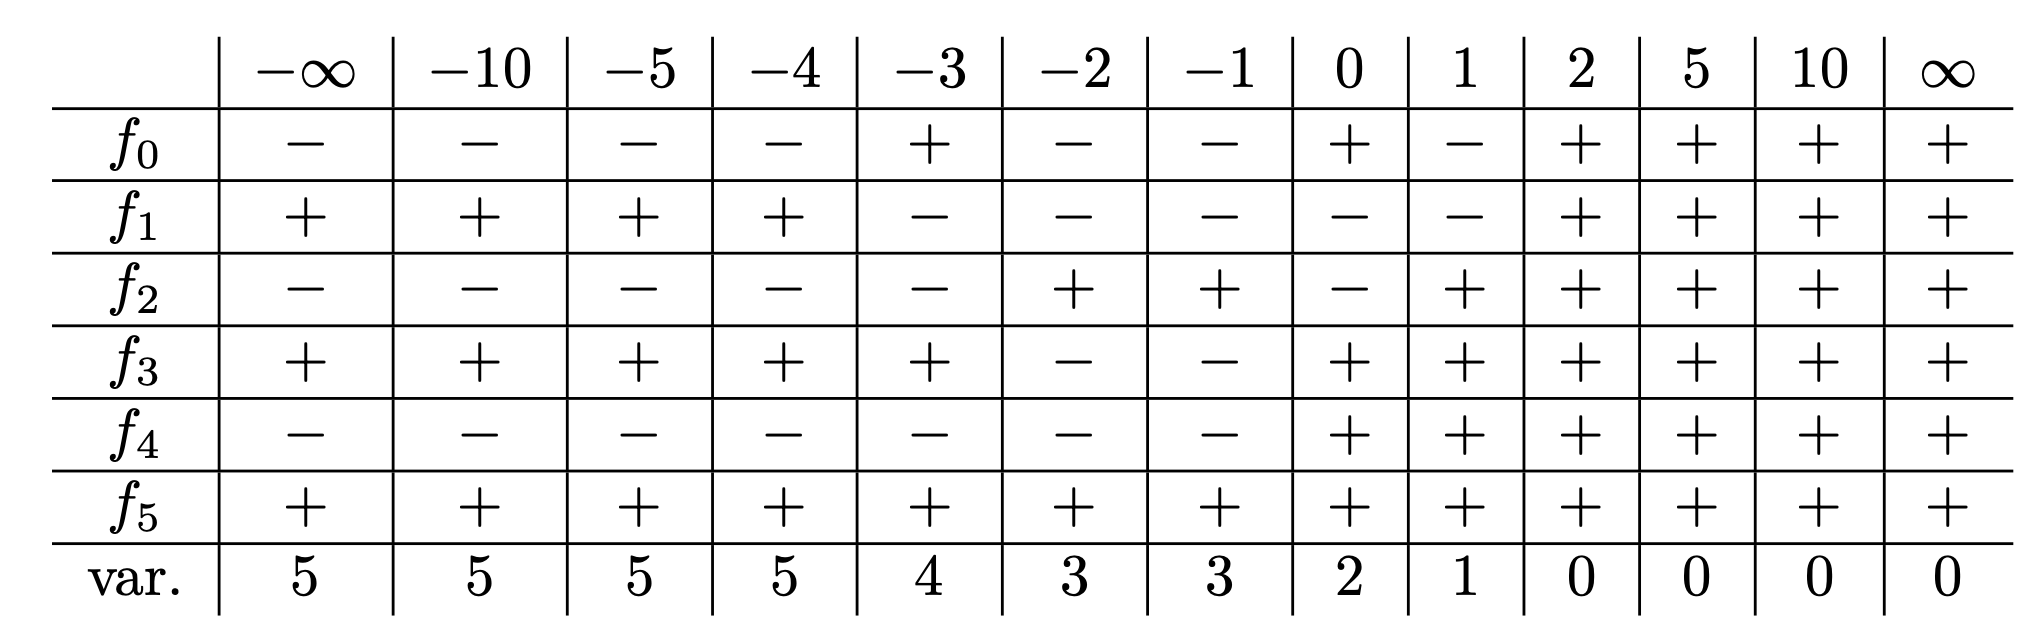
\includegraphics[width=10cm]{sturm-figure}}
  \begin{itemize}
  \item So roots between (-4, -3), (-3, -2), (-1,0), (0,1) and (1,2)
  \end{itemize}
\end{frame}


\section{Deflation}

\begin{frame}
  \frametitle{Deflation}
  \begin{itemize}
  \item Once you have a root r you can deflate a polynomial
    \[
      p(x) = (x-r) q(x)
    \]
  \item As the degree decreases the complexity of root finding is simplified. 
  \item One can use Horner's scheme
    \[
      p(x) = b_0 + (x-r)(b_n x^{n-1} + \ldots + b_2 x + b_1)
    \]
    as r is a root $b_0 = 0$ so
    \[
      q(x) = b_n x^{n-1} + \ldots + b_2 x + b_1
    \]
  \end{itemize}
\end{frame}

\begin{frame}
  \frametitle{Horner's Scheme Example}
  \begin{itemize}
    \item Lets take a simple example:
          \[
          p(x) = x^{3} - 2 x^{2} - 4 x + 3
          \]

    \item We can rewrite the polynomial as:
          \[ p(x) = ((x -2) x - 4) x +3 \]

    \item where each linear term can be evaluated individually
  \end{itemize}
\end{frame}

\section{Newton's Method}

\begin{frame}
  \frametitle{Newton's Method}
  \begin{itemize}
  \item Remember we can do root search/refinement
    \[
      x_{k+1} = x_k - \frac{p(x_k)}{p'(x)}
    \] we know that
    \[
      p(x) = p(t) + (x-t) q(x)
    \]
    So p'(t) = q(t) or
    \[
      q(x) = \frac{p(x)}{x-t}
    \]
  \item If p(x) has double roots it could be a challenge
  \end{itemize}
\end{frame}

\section{M{\"u}ller's Method}

\begin{frame}
  \frametitle{M\"ullers Method}
  \begin{itemize}
  \item Newton's Method is local and sensitive to seed guess    
  \item M\"ullers method is more global
  \item Based on a quadratic interpolation
  \item Assume you have three estimates of the root: $x_{k-2}, x_{k-1}, x_k$
  \item Interpolation polynomial
    \[
      p(x) = f(x_k)
      + f[x_{k-1}, x_k](x-x_k)
      + f[x_{k-2}, x_{k-1}, x_k](x-x_k)(x-x_{k-1})
    \]
  \item Using the equality
    \[
      (x-x_k)(x-x_{k-1}) = (x-x_k)^2 + (x-x_k)(x_k-x_{k-1})
    \] we get
    \[
      p(x) = f(x_k) + b (x-x_k) + a (x-x_k)^2
    \]
    which we can solve for p(x) = 0
  \end{itemize}
\end{frame}

\section{Summary}

\begin{frame}
  \frametitle{Summary}
  \begin{itemize}
  \item Frequently using a polynomial refactorization is more stable
  \item A way to compress data into a semantic form
  \item For lower order polynomials we have closed for solutions
  \item We can use Descartes rules, ... to bracket roots
  \item We can find roots and reduce polynomials
  \item Newton's method is a simple local rule, but could be noisy
  \item Mullers method is a way to solve it more generally 
  \item Lots of methods available for special cases
  \end{itemize}
\end{frame}

\end{document}

%%% Local Variables:
%%% mode: latex
%%% TeX-master: t
%%% End:
